
\chapter{Requirements and Architecture}
In order to come up with detailed requirements and a corresponding architecture an explorative process had to be used. The initial, overall objective was to createa general-purpose DDoS visualization system that focuses on data available in the DDoSDB dataset. In literature there one can find processes on how to derive an appropriate visualization for a defined problem, such as the following data analysis step from Marty\cite{appliedsecurityvisualization}:
\begin{enumerate}
    \item Define the problem to become aware of which questions need to be answered by the final visualization.
    \item Assess the available data to determine how it can be used and how it might need to be extended.
    \item Parse and filter the available data to extract the relevant information
    \item Determine which visual properties such as shape or size are needed
    \item Determine the view of the graph that was created in the previous step. This includes transformatinos such as scale or zooming.
    \item Interpret the graph and answer the initial question
\end{enumerate}

Since this process is targeted at solving a specific problem and our objective was the development of a general-purpose visualization system we adapted it as is described in the remaining sections of this chapter. First, we analysed the information that can be extract from various network captures from DDoSDB. This also included the determination of their scale and possible tools for data extraction. The outcome of this step was a general understanding on how the data needs to be parsed, aggregated and or filtered to create a general-purpose visualization system. This constitutes a "bottom-up approach" where we first analyse the data and parse it in the most generic way that enables the information to be used with as many visualizations as possible while still maintaining technical feasibility for large datasets.

>> How did we come up with requirements?? 

Given the requirements to such a system and the understanding of available information and scale of the data sets we then created the initial architecture.

\section{Analysis of Data Sets}
Before defining detailed use-cases available data was explored to determine feasible requirements, visualizations and implementations. To be more specific, a proof of concept data mining tool was built to answer the questions that needed to be cleared before progressing. The following subsections describe the questions that were supposed to be answered by the Proof of Concept and their results. With these results in hand an initial brainstorming session about possible use-cases done we were able to synthesize all information. The result is the use-cases that are supposed to be as abstract as possible to be inline with the overall objective of building a general-purpose platform whose prototypical implementation can be considered technically feasible.
The scope of the POC was to write a data miner that can provide at least the same functionality as can be obtained from the fingerprints that are available in DDoSDB.


\subsection{Libraries and Tooling}

\textit{What libraries exist and which features do they provide?}   

   Different tools and libraries were evaluated such as tsflow a CLI tool, node\_pcap a JavaScript based wrapper around libpcap and pkts, which is a parser written purely in Java.
    The Java library seemed to provide the best performance but for simple prototyping the Node.js based library was chosen. It provided parsing of protocols up until the application layer (app layer not included?) and heavily relies on libpcap. Support for stream processing in Node.js and the event-driven nature of JavaScript made the implementation feel quite "natural" and easy to read.
    Using node\_pcap it was possible to create the same information as provided in the DDoSDB dataset. Initially we suspected that we would run into performance problems especially when using very large datasets, which turned out not to be the case. This was due to the ease of implementation using stream processing which would make the POC scale easier with large sets. The duration of mining was also surprisingly good. This was tested by profiling the application when mining the largest dataset we could find on DDoSDB. This revealed that it only took seconds and that a majority of time was spent in the native libpcap module. This can be explained in that node\-pcap is merely a wrapper around libpcap. Figure \ref{fig:profiling} shows the result of profiling the miner. We thus conclude that node\_pcap provides all required functionality and that writing the miner in a way that it scales to larger datasets will be straightforward.
    
    \begin{figure}[profiling]
    \centering
    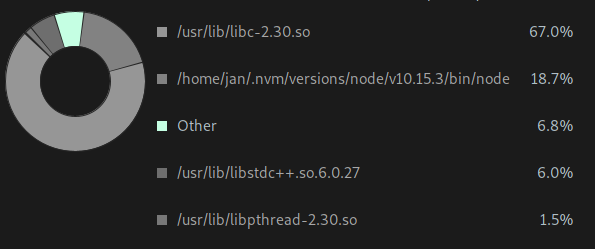
\includegraphics[width=10cm]{images/profiling.png}
    \caption{Profiling the data miner with a 15MB network capture as input.}
    \label{fig:profiling}
\end{figure}

> Describe implementation for further reeferences
    
\subsection{Information granularity?}
\textit{What information is contained in the network capture data sets? Which protocols and levels are sensible to analyse?
}

As a source for possible datasets the DDoSDB database was chosen. The reason for this are the features it provides as stated in section \ref{ddosdb}. The main benefit was direct access to network capture files that are already classified and in various sizes. This made it easy to see which information can be obtained in different attacks, such as for example, the payload of an ICMP packet. Since it is very simple to create a network capture of a "normal state" it was simple to compare the analysis of both cases.
Using the network capture files and a WHOIS service with the implemented proof of concept we were able to recreate the fingerprints from DDoSDB along with some additional information. The remainder of this section describes the data that can be extracted and an assessment if and how it is useful to collect for a visualization system:
\subsubsection{PCAP}
The first packet is a PCAP wrapper around the network-access level packet. It contains information such as \textbf{packet length} and a \textbf{timestamp} in seconds and microseconds. It is worth to note that this data needs to be interpreted on the place where it was captured.
Both of these properties are important to gather in order to compute the average packet length and attack start and duration.
\subsubsection{Network access layer}
In the payload of the PCAP packet one usually finds an Ethernet packet. Other network-layer protocols would be possible but only Ethernet packets were observed in the network captures.
The following information can be extracted from Ethernet packets:
\begin{itemize}
\item Destination and Source MAC addresses
\item Network-layer protocol
\item vlan ID
\end{itemize}
Since the information is very low-level and does not convey important semantics about any of the most frequent DDoS attack types we don't consider any of the information useful to store except for the Internet protocol that would be considered in the next subsection.
\subsubsection{Internet layer}
This was the first layer where multiple protocols were observed, naturally those would be IPv4 and IPv6. The network captures within DDoSDB were almost entirely based on IPv4 which is why this was focused on:
\begin{itemize}
\item Source and destination address
\item Version
\item TTL
\item DiffServ
\item Length
\item Transport-layer protocol
\item Version
\item checksum
\end{itemize}
     Except for checksums and transport-layer protocol, which was considered on the next layer, all properties could be sensible to mine.
     For some attacks the number of involved source addresses was very large, so large that fingerprints from DDoSDB would easily be larger than five megabytes. The problem with that is that it is difficult to work with in a front-end web application and it would be hard to visualize. For datasets that exceed some threshold of number of IP addresses aggregation would likely be required. This aggregation could be done based on arbitrary prefix aggregation, country or autonomous system.
     Other properties that are also sensible to aggregate would be TTL and length.
     \subsubsection{Transport layer}
In the transport layer two protocols were frequently observed: UDP and TCP.
Common to the two are the following fields:
\begin{itemize}
    \item Source and destination port
    \item Checksum
\end{itemize}
The packets using the TCP protocol also showed the following fields:
\begin{itemize}
    \item Acknowledgement number
    \item Sequence number
    \item Header length
    \item All six single-bit flags
    \item Window size
    \item Urgent Pointer
\end{itemize}
Source and destination port are definitely valueable to gather information on the application protocol being attacked. The flags would also be easy to aggregate over and give insight over the TCP state.

\subsection{Application layer}
The library that was used to parse packets does not contain a parser for application-level protocols. This means that to analyse this layer one has the protocol number and a buffer containing the payload. Perhaps it is already enough to aggregate over the type of protocols used. However the final implementation should definitely be easily extendable with new parsers for such protocols. For example, Node.js offers a performant and widely used HTTP parser which could be used to further gain insight about the application-level attack.
     
    \subsection{Scale and Schema of data}\label{scaleandschema}
\textit{    Are there consequences of the size and schema of the data with respect to visualizations? Can some technical challenges be determined?
}

    The reason why this question needs to be answered before designing visualizations is that depending on the size and distribution of the attributes that need to be visualized the visualization will either provide little value or be technically difficult. For example, consider an attack with 100'000 source IP addresses. Storing and fetching these addresses from a server to a web application will be taxing. Even if this were possible, there will hardly be a visualization that will provide insight while visualizing all 100'000 IP addresses. The answer to this question should define if aggregation of such attributes needs to be done and how.
    This is a technical challenge that can be taken for granted since network capture are technically unbound in size. This will also imply technical challenges for the mining of the source data since not the whole source and analysed data can be kept in memory.
    These challenges were observed while implementing the proof of concept. We assume that the following countermeasures will become important:
    \begin{itemize}
    \item     Applying \textbf{Big data techniques} to mine the source data will be very important to guarantuee that the data miner is technically capable of handling very large network capture files
\item Just looking at the fingerprints of the larger network captures in DDoSDB reveals that some of these JSON files are multiple megabytes in size. This both technically challenging to transfer and render and hard to interpret. However not only the size of these summaries is a problem, the fact that all information is contained in a single JSON file would lead to overfetching when used for different visualization. Overfetching refers to the problem of having to retrieve more data than being required by the client. Our solution to reducing the size and getting rid of overfetching is to create different resulting files for different visualizations. In a sense we would try to "\textbf{fan out}" the results over multiple files for improved scalability. For example, this could mean that for a time-series analysis of an attack we would create fixed-sized intervals and then create JSON files for each time interval. For other visualizations that would deal with more abstracted information we would also create single JSON files that have the only purpose to be used in that visualization. For example, a visualization a bar chart showing the top five autonomous systems used in an attack would only have to fetch a very small, dedicated JSON file containing said information.
\item Another solution to the aforementioned dilemma with very large results is to \textbf{aggregate} them. Ideally, this should be possible in a dynamic and user-defined way. For example, if an attack is executed from five source IP addresses, then this is technically possible and sensible to store as result and show in a visualization. However for hundreds or thousands of IP addresses either this visualization should be disabled or the underlying data could be aggregated to larger prefixes.
\item To enable the threshold where data will be aggregated more aggressively such a \textbf{user input} has to be implemented into the frontend of the webapplication.
\item Using a WHOIS service to query additional data about the source IP addresses does not scale up if more than a few thousand IP addresses need to be analysed. This is due to many WHOIS service providers being unwilling to deal with bulk requests of this size. Additionally, such requests would increase the duration of the data mining since it has to be transferred over the network. A local database needs to be considered as described in \ref{enrichingthedata}
\end{itemize}
    
    \subsection{Enriching the data}
\label{enrichingthedata}    \textit{Given the information that can be extracted, how can it be enriched? Which information makes sense to complement the network capture information with and how can it be obtained?}
    
In order to rebuild the functionality provided by the DDoSDB data miner, we need to provide the country and autonomous system number (asn) for each source IP address.
In the proof of concept implementation we used a WHOIS service provided by Team Cymru. This service supports bulk requests for WHOIS requests but is only willing to answer requests containing "(..) a few thousand" IP addresses \cite{teamcymru}. This along with the latency introduced by fetching the results over the network make this solution impracticable. For this, we intend to use the Geolite2 databases which are often used for geolocation of IP addresses. These datasets are interesting to us since they can be used locally and they have different datasets through which we could retrieve the ASN, country, city and belonging prefix for a source IP address \cite{geolite2}.

    
    \subsection{Aggregating the data} 
\textit{Given the information that can be extract how can or does it need to be aggregated?
}    

Section \ref{scaleandschema} described the necessity to aggregate in order to improve technical scalability and to make the visualizations sensible.
To visualize information with little abstraction, such as for example the source IPs for a certain time period, we will create a small data set containing just the relevant properties for that time interval.
For information with higher abstraction, such as for example visualizing overall metrics we follow the same strategy of creating a dataset for the visualization.
    \subsection{Fitting visualizations}
\textit{Given all the information that can be obtained, which visualizations are sensible?
}

We already established that the datasets need to be decoupled depending on visualization. To build a general purpose visualization platform it would be a good strategy to build a data miner that can easily be extended and then build visualizations and parsers for the most common attack types.
    \subsection{Constraints} 
\textit{Which constraints on the user input make sense? Which data sets make sense (e.g. location of recording)
}

If the application can deal with large datasets there should still be a limit for the size of input files since we don't know in which setting the application would be used. We think it makes sense to allow a user to define such a threshold in the application. Other constraints that are related to the visualizations, for example hiding certain outliers should be considered when designing the visualization.
In a first step it makes sense to write parsers only for network capture files, ideally from the DDoSDB database.
    
    \subsection{Frequent problems described in literature} 
    \textit{Literature describes that frequent problems are "Incomplete Information" and "Source / Destination Confusion". Are such problems relevant and if yes how can they be mitigated?}
    
    Detecting whether a dataset is incomplete is quite a difficult task since the proposed solution is not supposed to act as a classification or intrusion detection system. We therefore have to assume that we work with sane network capture files, which seems fair? since this data was already pre-processed by the DDoSDB\-cli and since network capture files are considered as rawest, compared to for example flow capture files \cite{appliedsecurityvisualization}.
    What is likely to happen and feasible to detect would be errors introduced when aggregating or extending the data. This would need to be indicated to the user somehow. For example, consider the case where we compute the top five autonomous systems used for an attack. If some of the IP addresses found in the parsed network captures can not be assigned to an autonomous system this information needs to be made aware to the user. Otherwise the information visualized will be distorted.
    The source destination problem is already mitigated to a certain degree since the destinations in the network capture files have been anonymised. What remains important is keeping a consistend naming and documentation throughout the data model up until the user interface.
    


\section{User Stories}
To elicit requirements for the tool and shape the direction this project will take, user stories were created. Three stakeholders were defined: \emph{Researcher}, \emph{Network Operator} and \emph{Professor}.
The table \ref{table:1} is an example of referenced \LaTeX elements.
\begin{table}[]
\centering
\begin{tabular}{|p{1.1cm}|p{12cm}|}
\hline
\textbf{ID} & \textbf{Description} \\ \hline

US 1         & As a professor user I want to use the application from a browser without installing additional software, because this way I can access the service from various devices.\\ \hline
US 1         & As a researcher I want to be able to host the application on my own machine and use it in a private environment, so I can make changes to the platform and test them.\\ \hline
US 3         & As a network operator I want the system to prioritize support for packet capture files, rather than network flow data, since packet captures provide a much more raw overview of an attack. \\ \hline
US 2         & As researcher, professor and network operator, I want to upload a PCAP file to have it analyzed and  visualized by the application. PCAP files should be accepted from DDoSDB or directly from network capture software.\\ \hline
US 2         & As a network operator, I want to be able to feed network data directly into the application, to monitor my network in real time.\\ \hline
US 3         & As a network operator, I want to upload other file types, since my packet capture system uses a different file structure than PCAP\\ \hline
US 4         & As a researcher and network operator, I want to be able to extend the platform by writing parsers/analysers for additional file types\\ \hline
US 5         & As a researcher I want to be able to extend the platform by extending the visualization capabilities of the application\\ \hline
US 6         & As a network administrator I want to have source IPs clustered by Attributes such as ISP, country or Prefixes to have a better overview of where an attack came from. This implies that additional information to the network capture is gathered.\\ \hline
US 7         & As a researcher, professor and network operator I want to be able to replay an attack using configurable time controls such as play/pause buttons or a time line. To inspect an attack in detail.\\ \hline
US 8         & As a network operator I want to be able to aggregate metrics of a PCAP file, such as the rate of incoming packets per second, number of incoming connections, etc. to find out high level information and conclusions about an attack as a whole.\\ \hline
US 9         & As a network operator I want to switch between simple visualizations with limited information and more complicated ones that are more detailed, so when I have to inform a higher up who is not very technically skilled I can present him simple visulaizations that he understands.\\ \hline
US 10        & As the researcher that hosts the platform, I want to access preferences of the application using an admin panel. This includes functionality like deleting data sets.\\ \hline
US 11        & As a professor user I want the application to come bundled with data sets that clearly show different attack types to show students what they look like and how they differ in appearance.\\ \hline
US 12        & As a researcher I want to be able to contact the CSG or maintainers of the platform, for example to suggest or discuss pull requests to the project.\\ \hline
US 13        & As a professor I want to be able to let students detect the type of attack by having the same packet capture plotted on different visualizations. The attack patterns of the most common DDoS attack types in 2019 should thus be covered by the visualizations\footnotemark. This includes UDP floods, HTTP-based attacks, SYN flood attacks, port scans and ICMP attacks.\\ \hline
US 14       & As a network operator, I want a visualization software that is agnostic to the type of attack or location where the attack was recorded. This stands in contrast with other tools such as Firewalls that have implemented visualizations as an afterthought which are specialized.\cite{appliedsecurityvisualizations}.\\ \hline
US 14       & As a researcher I want to be inspired to try new visualization techniques, since this is often required to find new patterns in network logs\cite{appliedsecurityvisualizations}. This requires that one can easily add, combine or adapt new visualizations to find new patterns in network logs as well as one can quickly try different visualizations for the same attack.\\ \hline
US 15       & As a network operator who is responsible for reporting to (non-technical) management I want that there are very high-level visualizations for all types of attacks. This is a requirement since one often has less than 60seconds to get a message to a non-technical person\cite{appliedsecurityvisualizations}. This will require aggregations as described in US 8.\\ \hline
US 15       & As a network operator who is responsible for the historical analysis of attacks I want to have detailed visualizations targeted at technical audiences, to draw conclusions about potential threats that might affect our network.\cite{appliedsecurityvisualizations}.\\ \hline
US 15       & As a researcher that  wants to use the visualization in papers, i want to be able to exprt the visualizations in PDF and image formats.\cite{appliedsecurityvisualizations}.\\ \hline
US 15       & As a researcher and network operator I want the application to work with very small and very large data sets. This will likely involve that the application is aware of the size of data sets and its effects on visualizations\cite{appliedsecurityvisualizations}. For example, the visualization of a all source IP addresses will require the aggregation into classes or prefixes if there are hundreds of thousands of addresses.\\ \hline
US 17       & As a researcher I want that visualizations are categorized by the attack pattern they are likely to indicate and required technical understanding as described in US-9. It should be easy to filter and select these visualizations.\\ \hline
US 18       & As a professor performing network security workshops, I work with different customers. The hardware and software that they use varies greatly which is why the application should work with all modern browsers and on slower hardware.\\ \hline
US 19       & As a researcher I want to get certain statistics that span over multiple attacks. For example, given a set of network captures, what was the most common protocol used?\\ \hline
US 20      & As a researcher associated with DDoSDB I want that the application is fully integrated with DDoSDB. This covers that network captures can directly be fed to the visualisation system without downloading them or that raw network captures that have been pre-processed can be uploaded to the DDoSDB data set.\\ \hline
US 20      & As a professor that presents the visualizations in presentations and lectures, I want to save and retrieve my setups and retrieve them in, so I don't have to recofigure a setup from scratch everytime\\ \hline
US 20      & As a reseracher i want to have an overview page for each dataset where I can see general information about the set such as description and high level statistics.\\ \hline

\end{tabular}
\caption{User Stories that influenced the direction and functionality of the application}
\label{table:1}
\end{table}               





\begin{table}[]
\centering
\begin{tabular}{|p{1.1cm}|p{12cm}|}
\hline
\textbf{ID} & \textbf{Description} \\ \hline

US 2         & As researcher, professor and network operator, I want to upload a PCAP file to have it analyzed and  visualized by the application. PCAP files should be accepted from DDoSDB or directly from network capture software.\\ \hline

US 4         & As a researcher and network operator, I want to be able to extend the platform by writing parsers/analysers for additional file types\\ \hline

US 7         & As a researcher, professor and network operator I want to be able to replay an attack using configurable time controls such as play/pause buttons or a time line. To inspect an attack in detail.\\ \hline
US 15       & As a researcher and network operator I want the application to work with very small and very large data sets. This will likely involve that the application is aware of the size of data sets and its effects on visualizations\cite{appliedsecurityvisualizations}. For example, the visualization of a all source IP addresses will require the aggregation into classes or prefixes if there are hundreds of thousands of addresses.\\ \hline

\end{tabular}
\caption{User Stories that influenced the direction and functionality of the application}
\label{table:1}
\end{table} 





\begin{table}[]
\centering
\begin{tabular}{|p{1.1cm}|p{12cm}|}
\hline
\textbf{ID} & \textbf{Description} \\ \hline

US 1         & As a professor user I want to use the application from a browser without installing additional software, because this way I can access the service from various devices.\\ \hline
US 11        & As a professor user I want the application to come bundled with data sets that clearly show different attack types to show students what they look like and how they differ in appearance.\\ \hline
US 13        & As a professor I want to be able to let students detect the type of attack by having the same packet capture plotted on different visualizations. The attack patterns of the most common DDoS attack types in 2019 should thus be covered by the visualizations\footnotemark. This includes UDP floods, HTTP-based attacks, SYN flood attacks, port scans and ICMP attacks.\\ \hline
US 18       & As a professor performing network security workshops, I work with different customers. The hardware and software that they use varies greatly which is why the application should work with all modern browsers and on slower hardware.\\ \hline
US 20      & As a professor that presents the visualizations in presentations and lectures, I want to save and retrieve my setups and retrieve them in, so I don't have to recofigure a setup from scratch everytime\\ \hline

\end{tabular}
\caption{User Stories that influenced the direction and functionality of the application}
\label{table:1}
\end{table} 



\begin{table}[]
\centering
\begin{tabular}{|p{1.1cm}|p{12cm}|}
\hline
\textbf{ID} & \textbf{Description} \\ \hline

US 1         & As a researcher I want to be able to host the application on my own machine and use it in a private environment, so I can make changes to the platform and test them.\\ \hline
US 5         & As a researcher I want to be able to extend the platform by extending the visualization capabilities of the application\\ \hline
US 10        & As the researcher that hosts the platform, I want to access preferences of the application using an admin panel. This includes functionality like deleting data sets.\\ \hline
US 12        & As a researcher I want to be able to contact the CSG or maintainers of the platform, for example to suggest or discuss pull requests to the project.\\ \hline
US 14       & As a researcher I want to be inspired to try new visualization techniques, since this is often required to find new patterns in network logs\cite{appliedsecurityvisualizations}. This requires that one can easily add, combine or adapt new visualizations to find new patterns in network logs as well as one can quickly try different visualizations for the same attack.\\ \hline
US 15       & As a researcher that  wants to use the visualization in papers, i want to be able to exprt the visualizations in PDF and image formats.\cite{appliedsecurityvisualizations}.\\ \hline
US 17       & As a researcher I want that visualizations are categorized by the attack pattern they are likely to indicate and required technical understanding as described in US-9. It should be easy to filter and select these visualizations.\\ \hline
US 19       & As a researcher I want to get certain statistics that span over multiple attacks. For example, given a set of network captures, what was the most common protocol used?\\ \hline
US 20      & As a researcher associated with DDoSDB I want that the application is fully integrated with DDoSDB. This covers that network captures can directly be fed to the visualisation system without downloading them or that raw network captures that have been pre-processed can be uploaded to the DDoSDB data set.\\ \hline
US 20      & As a reseracher i want to have an overview page for each dataset where I can see general information about the set such as description and high level statistics.\\ \hline

\end{tabular}
\caption{User Stories that influenced the direction and functionality of the application}
\label{table:1}
\end{table} 

\begin{table}[]
\centering
\begin{tabular}{|p{1.1cm}|p{12cm}|}
\hline
\textbf{ID} & \textbf{Description} \\ \hline

US 3         & As a network operator I want the system to prioritize support for packet capture files, rather than network flow data, since packet captures provide a much more raw overview of an attack. \\ \hline
US 2         & As a network operator, I want to be able to feed network data directly into the application, to monitor my network in real time.\\ \hline
US 3         & As a network operator, I want to upload other file types, since my packet capture system uses a different file structure than PCAP\\ \hline
US 6         & As a network administrator I want to have source IPs clustered by Attributes such as ISP, country or Prefixes to have a better overview of where an attack came from. This implies that additional information to the network capture is gathered.\\ \hline
US 8         & As a network operator I want to be able to aggregate metrics of a PCAP file, such as the rate of incoming packets per second, number of incoming connections, etc. to find out high level information and conclusions about an attack as a whole.\\ \hline
US 9         & As a network operator I want to switch between simple visualizations with limited information and more complicated ones that are more detailed, so when I have to inform a higher up who is not very technically skilled I can present him simple visulaizations that he understands.\\ \hline
US 14       & As a network operator, I want a visualization software that is agnostic to the type of attack or location where the attack was recorded. This stands in contrast with other tools such as Firewalls that have implemented visualizations as an afterthought which are specialized.\cite{appliedsecurityvisualizations}.\\ \hline
US 15       & As a network operator who is responsible for reporting to (non-technical) management I want that there are very high-level visualizations for all types of attacks. This is a requirement since one often has less than 60seconds to get a message to a non-technical person\cite{appliedsecurityvisualizations}. This will require aggregations as described in US 8.\\ \hline
US 15       & As a network operator who is responsible for the historical analysis of attacks I want to have detailed visualizations targeted at technical audiences, to draw conclusions about potential threats that might affect our network.\cite{appliedsecurityvisualizations}.\\ \hline

\end{tabular}
\caption{User Stories that influenced the direction and functionality of the application}
\label{table:1}
\end{table} 

As mentioned in US 16 and US 18 it is important that the application can handle small, as well as very large data sets. This requires that, depending on the visualization, thresholds have to be set for certain attributes that define when it will be clustered or used differently in a visualization. For example for smaller data sets it might be possible to draw all source IPs and their hosts, but for a larger set it may require a lot of CPU power that results in a visualization that it illegible and unneccesarily complex. This fact influences the way we pre-process data sets in order to have them visualized in the application as fast as possible. Another feature that is affected of this selective pre-processing, is the toggle that switches between simple visualizations only and more detailed and technical views. For a non-technical user that wants a broad overview of an attack, we assume that 1) he is less inclined to wait until a visualization has loaded and 2) simple charts, such as bar charts and graphs that display precalculated metrics will suffice. This goes well in hand with our problem of differently sized data sets and the need of calculating metrics in advance.

\footnotetext{US 13: UDP floods and HTTP-based attacks have been the most common type of DDoS attacks by the end of 2018\cite{hostingtribunal.com}.}

\section{Requirements}
\subsection{Infrastructure}
\begin{table}[]
\centering
\begin{tabular}{|p{1.1cm}|p{12cm}|}
\hline
\textbf{ID} & \textbf{Description} \\ \hline
RQ 1 & The application will be hosted as a web application and will be accessible with all modern browsers.\\ \hline
RQ 2 & To store the uploaded data sets, a XXXXX database will be used.\\ \hline
RQ 3 & Smaller data sets can be stored in browser-memory?????.\\ \hline
RQ 4 & The repository for the source code will be made open source and extensible by other parties.\\ \hline

\end{tabular}
\caption{Infrastructure Requirements that were elicited from the User Stories}
\label{table:2}
\end{table}

\subsection{Application Features}
\begin{table}[]
\centering
\begin{tabular}{|p{1.1cm}|p{12cm}|}
\hline
\textbf{ID} & \textbf{Description} \\ \hline
RQ 5 & The application features a file upload functionality that accepts PCAP files either from a local source or from an URL/external location such as DDoSDB\\ \hline
RQ 5 & The upload dialog features a file format check, that checks whether the file is in a valid format to be further processed and visualized\\ \hline
RQ 5 & The dialog features a selection that lets the user define which miner/parser will be used for the data set he uploads. This influences the visualizations possible with the specific data set\\ \hline
RQ 5 & A description and a name can be added to a data set, so that it may be recognised later. Should no name be entered, a standardized naming scheme will be applied\\ \hline
RQ 5 & The application lets a user choose already uploaded data sets to visualize\\ \hline
RQ 5 & The application features an About/Contact node, where contact information about the CSG and GitHub links are presented.\\ \hline
RQ 5 & When opening the application, the user is presented with a short introduction about the application in form of an introductory text that explains the DDoS Visualizer and its features\\ \hline
RQ 5 & Since not all data sets are suited for every visualization on the platform, a selection of possible visualization methods is presented when selecting a data set. \\ \hline
RQ 5 & The name and description of a data set are also displayed when selecting a data set\\ \hline
RQ 5 & The list of available data sets, the upload button, as well as contact buttons are placed in a retractable sidebar that can be accessed and closed via a hamburger button and a cross button respectively\\ \hline
RQ 5 & The application features an export button that allows the visualization to be exported as an image or pdf file\\ \hline

\end{tabular}
\caption{Application Features that were elicited from the User Stories}
\label{table:3}
\end{table}

\subsection{Data Processing}
\begin{table}[]
\centering
\begin{tabular}{|p{1.1cm}|p{12cm}|}
\hline
\textbf{ID} & \textbf{Description} \\ \hline
RQ 1 &  The application should accept PCAP files, especially those available on DDoSDB\\ \hline
RQ 1 &  The uploaded files that fit the requirements will be converted into an generalized format that suits certain visualizations.\\ \hline
RQ 1 &  Depending on the size and complexity of the file, it may be shortened, summed up and matrics may be evaluated, so that large datasets are still eligible to be visualized\\ \hline
RQ 1 &  \\ \hline
RQ 1 &  It should be possible to extend the accepted file formats, by writing parsers/miners that convert the file into the accepted generalized format produced by the data processor\\ \hline

\end{tabular}
\caption{Data Processing Requirements that were elicited from the User Stories}
\label{table:2}
\end{table}

\subsection{User Flows}
\begin{table}[]
\centering
\begin{tabular}{|p{1.1cm}|p{12cm}|}
\hline
\textbf{ID} & \textbf{Description} \\ \hline
RQ 1 & When opening the application, a user can open and close the sidebar\\ \hline
RQ 5 & On an open sidebar he can click on an existing data set, that takes him the that data set's overview page\\ \hline
RQ 5 & When clicking on the 'Upload Data Set' button, the file upload dialog appears\\ \hline
RQ 5 & After uploading a data set the user gets redirected to the front page and the newly added data set is visible once it is finished processing\\ \hline
RQ 5 & When clicking on an entry in the 'About/Contact' section in the sidebar, it will open the respective link in a new tab\\ \hline
RQ 5 & On a data set's overview page, a user can select one of the available visualizations, that takes him to the visualization view\\ \hline

\end{tabular}
\caption{User Flow Requirements that were elicited from the User Stories}
\label{table:2}
\end{table}

\subsection{Visualizations}
\begin{table}[]
\centering
\begin{tabular}{|p{1.1cm}|p{12cm}|}
\hline
\textbf{ID} & \textbf{Description} \\ \hline
RQ 1 & On the visualization view for a data set, if available, filters are presented that modify the resulting visualization. For example a minimum number of connection tries can be defined in order to hide honest nodes.\\ \hline
RQ 5 & On the visualization view, if available time controls can be used to display a certain moment in the attack's history\\ \hline
RQ 5 & If a visualization has a history that can be accessed, a play and pause button can be pressed to view the progression of an attack at a certain speed\\ \hline
RQ 5 & When a visualization has been selected, additional visualizations can be selected using an 'Add' button. The chosen one will be placed below the existing visualization(s)\\ \hline
RQ 1 &  Every visualization comes with a 'Remove' button to remove said visualization from the stack\\ \hline
RQ 5 & One visualization requires the data to be processed in a way so that the source IPs of an attack can be traced to their respective ISPs, meaning they can be clustererd by ISP to see which operator might be inclined to implement certain restrictions in their network.\\ \hline
RQ 5 & Another way to cluster nodes would be by IP prefixes, to detect malicious subnets\\ \hline
RQ 5 & To make sense of multiple datasets and compare them, it should be possible to gather statistics and similarities about multiple datasets\\ \hline
RQ 5 & The platform should be extensible in terms of visualizations. A developer should easily be able to add more visualization to the platform.\\ \hline
RQ 5 & A visualization should be categorized into a simple and complex visualizations to make use of the toggle on the application that hides technical information for non-technical users\\ \hline
RQ 5 & The application should be able to clearly visualize common attack patterns such as UDP floods, HTTP-based attacks, SYn flood attacks, port scans and ICMP attacks.\\ \hline
RQ 5 & The visulaizations should offer general views on networks, regardless of the network of the original data-source.\\ \hline
RQ 1 &  Using the aggregated metrics and summarized data described in RQ???, high level vies of an attack should be available that tell the most important attributes of an attack and it's effect on the network.\\ \hline

\end{tabular}
\caption{Visualization Requirements that were elicited from the User Stories}
\label{table:2}
\end{table}

\section{Architecture}

\chapter{Design and Implementation}